\section{Architectural-Level Synthesis}
Trying to pass from logic to architectural level racecourse at higher level allow to see all possible options. Having less details, it possible work with higher complex circuit. You can decide to use a bigger block with high complexity at logic level, but the block that you have connected and improved don't allow to see a global improvement.\\
The motivations to raise abstraction level:
\begin{itemize}
\item Reduce specification of details
\item Extend designer base
\item Ease modifications and extensions
\item Reduce design time
\item Explore and optimize macroscopic structure
\end{itemize}
Architectural synthesis means constructing the macroscopic structure of a digital circuit, starting from behavioral models that can be captured by data-flow or sequencing graphs. The outcome of architectural synthesis is both a structural view of the circuit, in particular of its data path, and a logic-level specification of its control unit. The data path is an interconnection of  \textit{resources} (implementing arithmetic or logic functions), \textit{steering logic circuits}  (e.g., multiplexers and buses), that send data to the appropriate destination at the appropriate time and  \textit{registers}  or  \textit{memory arrays}  to store data.
\begin{figure}[H]
	 \centering
	 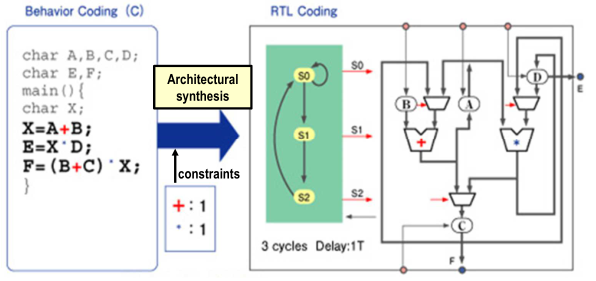
\includegraphics[height=50mm]{./Cap3/Images/Image01.png}
	 \caption[Optional caption]{Example of Architectural synthesis}
	 \label{fig:archSy}
\end{figure}

\subsection{Hardware and software compilation}
A \textit{software} compiler consists of a  front end  that transforms a program into an intermediate form  and a  back end  that translates the intermediate form into the machine code for a given architecture. The front end is language dependent, and the back end varies according to the target machine. Similarly, a \textit{hardware} compiler can be seen as consisting of a front end, an optimizer and a back end (Figure 3.16). The back end is much more complex than a software compiler, because of the requirements on timing and interface of the internal
operations.
\begin{figure}[H]
	 \centering
	 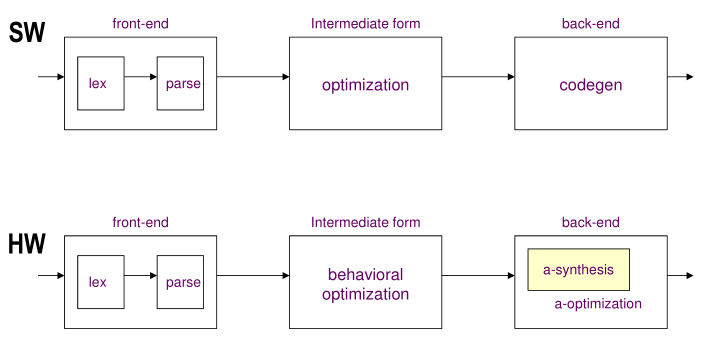
\includegraphics[height=50mm]{./Cap3/Images/Image02.png}
	 \caption[Optional caption]{Hardware and software compilation}
	 \label{fig:comp}
\end{figure}

\subsubsection{Compilation  Techniques}
The front end of a compiler is responsible for  \textit{lexical}  and  \textit{syntax} analysis, \textit{parsing}  and \textit{creation} of the intermediate form. Its first task is to verify that they satisfy the syntax rules of the language. The parser has knowledge of the grammar of the language and it generates a set of  parse trees.  A parse tree is a tree-like representation of the syntactic structure of a language. An example is shown in Figure \ref{fig:parseTree}. Syntactic errors, as well as some semantic errors are detected at this stage.
\begin{figure}[H]
	 \centering
	 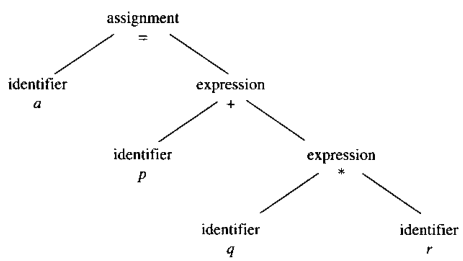
\includegraphics[height=50mm]{./Cap3/Images/Image03.png}
	 \caption[Optional caption]{Example  of  a  parse  tree  for  the statement  $ a  =  p  +  y  *  r $}
	 \label{fig:parseTree}
\end{figure}
Branching constructs can be used to model logic networks. A common way to exploit branching is by means of conditional assignments to a variable.  A  branching construct can be replaced by one logic expression, representing the disjunction of the possible assignments in conjunction with the test on the clause. When the branching construct does not specify an assignment for all values of the clause, the missing assignments represent  \textit{don't  care}  conditions on that variable. The compilation of hardware models at the architectural level involves a full \textit{semantic}, \textit{analyses}  that comprises  \textit{data-flow}  and  \textit{control-flow}  analyses.
\begin{figure}[H]
	 \centering
	 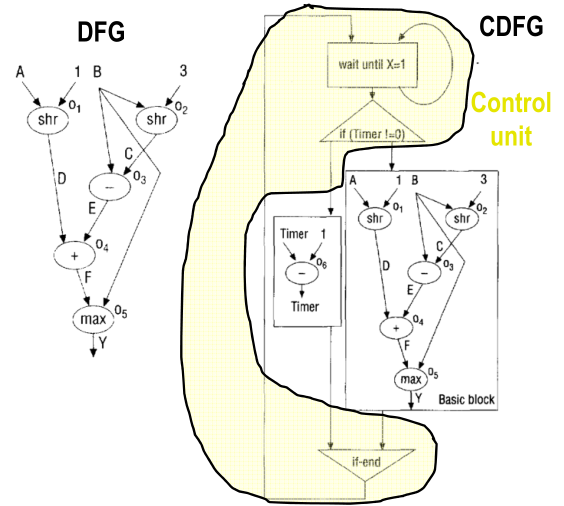
\includegraphics[height=50mm]{./Cap3/Images/Image04.png}
	 \caption[Optional caption]{Data-flow graph and Control-data-flow graph}
	 \label{fig:dataFlow}
\end{figure}

\subsubsection{Optimization Techniques}
Behavioral optimization is a set of transformations that minimize the amount of information needed to specify the partial order of tasks. It can be applied directly to the parse trees, or during the generation of the intermediate form.\\
Algorithms for behavioral optimization of  HDL  models can he classified as data-flow and control-flow
oriented.
\begin{itemize}
\item \textbf{DATA-FLOW-BASED TRANSFORMATIONS}: 
	\begin{itemize}
	\item \textit{Tree-height reduction}: This transformation applies to the arithmetic expression trees and strives to achieve the expression split into two-operand expressions, so that the parallelism available in hardware can be exploited at best. The simplest reduction algorithm uses the \textit{commutativity} and \textit{associativity} of the addition and multiplication. It permutes the operands to achieve subexpressions involving the same operator, which can be reduced by using the associative property. A  further refinement can be achieved by exploiting the \textit{distributive} property, possibly at the expense of adding an operation.
	\begin{figure}[H]
    \centering
    \begin{subfigure}[b]{0.4\textwidth}
        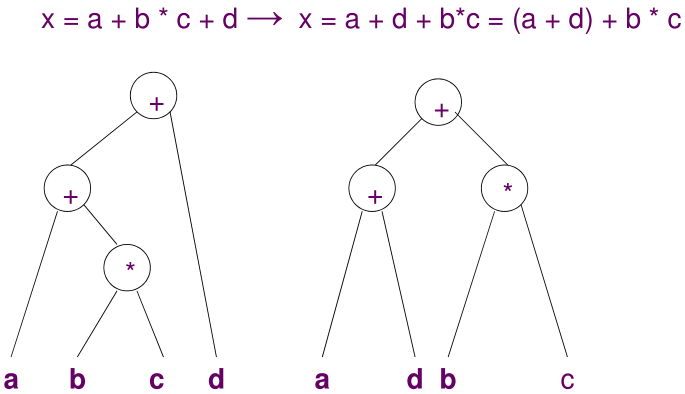
\includegraphics[width=\textwidth]{./Cap3/Images/Image05.png}
        \caption{using Commutativity and Associativity}
        \label{fig:comAss}
    \end{subfigure}
    \quad\quad\quad
    \begin{subfigure}[b]{0.4\textwidth}
        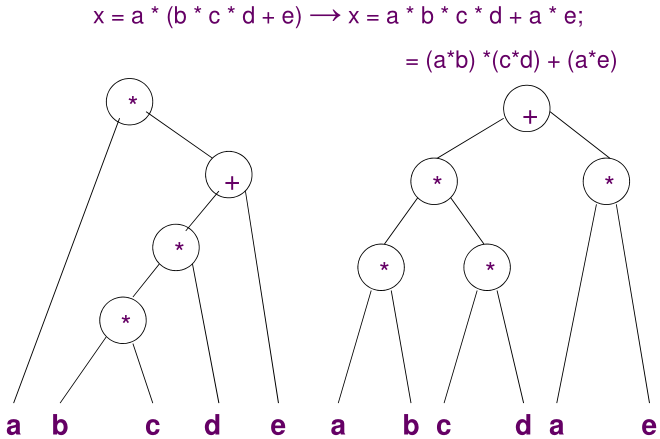
\includegraphics[width=\textwidth]{./Cap3/Images/Image06.png}
        \caption{using Distributivity}
        \label{fig:Dis}
    \end{subfigure}
	\end{figure}
	\item \textit{constant and variable propagation}:  \textit{Constant} propagation consists of detecting constant operands and pre-computing the value of the operation with that operand. Since the result may be again a constant, the new constant can be propagated to those operations that use it as input.
	\begin{figure}[H]
	 \centering
	 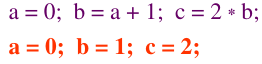
\includegraphics[width=0.25\textwidth]{./Cap3/Images/Image07.png}
	\end{figure}
	\textit{Variable} propagation consists of detecting the copies  of variables, i.e., the assignments like  x  =  y,  and using the right-hand side in the following references in place of the left-hand side. 
	\begin{figure}[H]
	 \centering
	 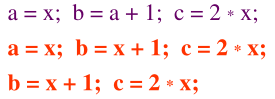
\includegraphics[width=0.25\textwidth]{./Cap3/Images/Image08.png}
	\end{figure}
	\item \textit{Common subexpression elimination}: The search for common arithmetic subexpressions relies in general on finding isomolphic patterns in the parse trees (\textit{Isomorphic}: if the subtree has the same inputs and the same operators). This step is greatly simplified if the arithmetic expressions are reduced to two-input ones. Then, this transformation consists of selecting a target arithmetic operation and searching for a preceding one of the same type and with the same operands.
	\begin{figure}[H]
	 \centering
	 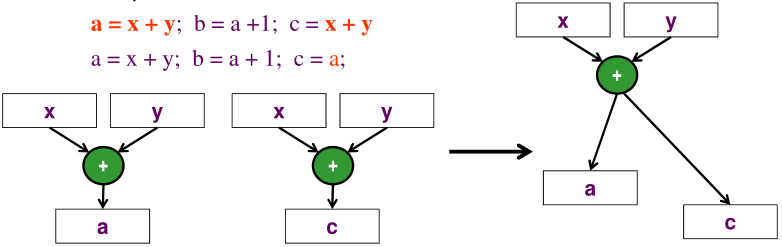
\includegraphics[width=0.4\textwidth]{./Cap3/Images/Image09.png}
	\end{figure}
	\item \textit{Dead code elimination};  Dead code consists of all those operations that cannot be reached, or whose result is never referenced elsewhere. 
	\begin{figure}[H]
	 \centering
	 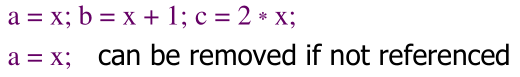
\includegraphics[width=0.4\textwidth]{./Cap3/Images/Image10.png}
	\end{figure}
	\item \textit{Operator strength reduction}:  Operator strength reduction means reducing the cost of implementing an operator by using a simpler one. 
	\begin{figure}[H]
	 \centering
	 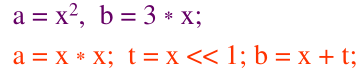
\includegraphics[width=0.3\textwidth]{./Cap3/Images/Image11.png}
	\end{figure}
	\item \textit{Code motion}:  Code motion often applies to loop invariants, i.e., quantities that are computed inside an iterative construct but whose values do not change from iteration to iteration. The goal is to avoid the repetitive evaluation of the same expression.
	\begin{figure}[H]
	 \centering
	 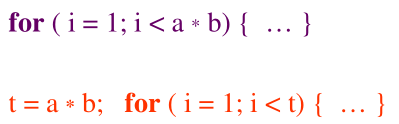
\includegraphics[width=0.3\textwidth]{./Cap3/Images/Image12.png}
	\end{figure}
	\end{itemize}
\item \textbf{CONTROL-FLOW-BASED TRANSFORMATIONS}:  The following transformations are typical of hardware compilers. In some cases these transformations are automated, in others they are user driven.
	\begin{itemize}
	\item \textit{Model expansion}: Consists in flattening locally the model call hierarchy. Therefore the called model disappears, being swallowed by the calling one. A  possible benefit is that the scope of application of some optimization techniques  is enlarged.
	\begin{figure}[H]
	 \centering
	 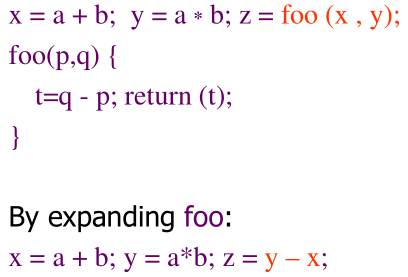
\includegraphics[width=0.3\textwidth]{./Cap3/Images/Image13.png}
	\end{figure}
	\item \textit{Conditional expansion}:  A  conditional construct can be always transformed into a parallel construct with a test in the end. Under some circumstances this transformation can increase the performance of the circuit. 
	\begin{figure}[H]
	 \centering
	 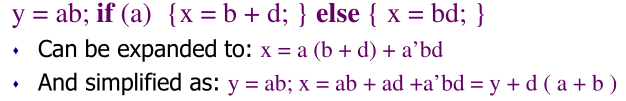
\includegraphics[width=0.5\textwidth]{./Cap3/Images/Image14.png}
	\end{figure}
	\item \textit{Loop expansion}:  Loop expansion, or unrolling, applies to an iterative construct with data-independent exit conditions. The loop is replaced by as many instances of its body as the number of operations. The benefit is again in expanding the scope of other transformations. 
	\begin{figure}[H]
	 \centering
	 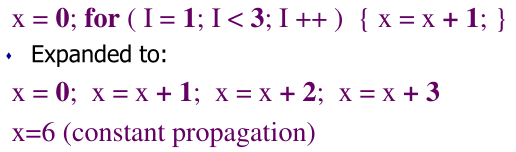
\includegraphics[width=0.4\textwidth]{./Cap3/Images/Image15.png}
	\end{figure}
	\end{itemize}
\end{itemize}

\subsection{Architectural synthesis and optimization}
Architectural synthesis means constructing the macroscopic structure of a digital circuit, starting from behavioral models that can be captured by data-flow or sequencing graphs. The outcome of architectural synthesis is both a structural view of the circuit, in particular of its data path, and a logic-level specification of its control unit.\\
Circuit implementations are evaluated on the basis of the following objectives: \textit{area}, \textit{cycle-time} (i.e., the clock period) and \textit{latency} (i.e., the number of cycles to perform all operations) as well as \textit{throughput} (i.e., the computation rate) in the case of pipelined circuits. Note that area and
performance measures can only be estimated at the architectural level, because just the macroscopic structure of the circuit is dealt with.  In  general, area and performance depend on the resources as well as on the steering logic, storage circuits, wiring and control.  A  common simplification is to consider area and performance as depending only on the resources. Circuits for which this assumption holds are called \textit{resource-dominated circuits}.\\
In the \textit{resource-dominated circuits} the estimation of the \textit{area} is sum of the area of the resources bound to the operations, mainly determined by  \textit{binding/sharing}. The estimation of the \textit{latency} is start time of the sink operation minus start time of the source operation, mainly determined by  \textit{scheduling}.\\
In the \textit{non resource-dominated circuits}, the \textit{area} is also affected by registers, steering logic, wiring and control. The \textit{cycle-time} is also affected by steering logic, wiring and (possibly) control.\\
Constraints in architectural synthesis can  be  classified into two major groups:  \textit{interface constraints}  and  \textit{implementation constraints}. Interface constraints are additional specifications to ensure that the circuit can be embedded in a given environment. They relate to the format and timing of the I/O data transfers. Implementation constraints reflect the desire of the designer to achieve a structure with some properties. Examples are area constraints and performance constraints, e.g.,  cycle-time  and/or  latency  bounds. A  different kind  of  implementation constraint is a resource \textit{binding constraint}. In the case of \textit{resource-dominated circuits}, the area is determined only by the resource usage. Hence bounding the number of resources is equivalent to imposing an upper bound on the area.
\bigskip \\
Performance constraints:
\begin{itemize}
\item Cycle-time
\item Latency of a set of operations
\item Time spacing between operation pairs\
\end{itemize}
Area constraints:
\begin{itemize}
\item Number and type of resources
\item Resource allocation
\item Partial binding
\end{itemize}

\subsection{The Temporal Domain: Scheduling}
We denote the execution delays of the operations by the set $ D = \lbrace d_{i};\:i=0,1,...,n \rbrace $. We define the  \textit{start time} of an operation as the time at which the operation starts its execution. The start times of the operations, represented by the set $ T = \lbrace t_{i};\:i=0,1,...,n \rbrace $,  are attributes of the vertices of the sequencing graph.  \textit{Scheduling}  is the task of determining the start times, subject to the precedence constraints specified by the sequencing graph. The \textit{latency} of a scheduled sequencing graph is denoted by $ \lambda $,  and it is the difference between the start time of the sink and the start time of the source, i.e.,  $ \lambda=t_{n}-t_{0} $.\\
A \textit{ scheduled sequencing  graph}  is a vertex-weighted sequencing graph, where each vertex is labeled by its start time.  A  schedule may have to satisfy timing and/or resource usage constraints. Different scheduling algorithms have been proposed, addressing unconstrained and constrained problems.
\begin{figure}[H]
	 \centering
	 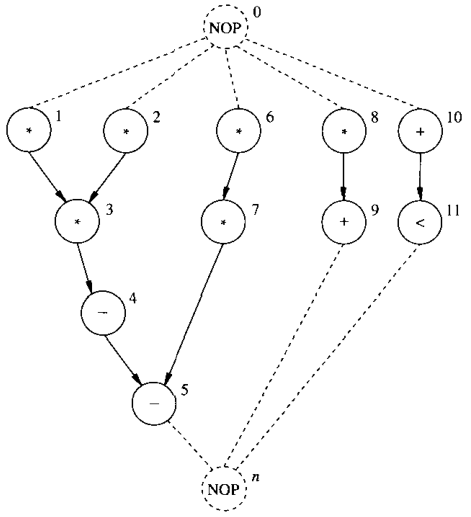
\includegraphics[width=0.5\textwidth]{./Cap3/Images/Image16.png}
	 \caption[Optional caption]{Sequencing  graph}
	 \label{fig:Sequ}
\end{figure}
\begin{figure}[H]
    \centering
    \begin{subfigure}[b]{0.4\textwidth}
        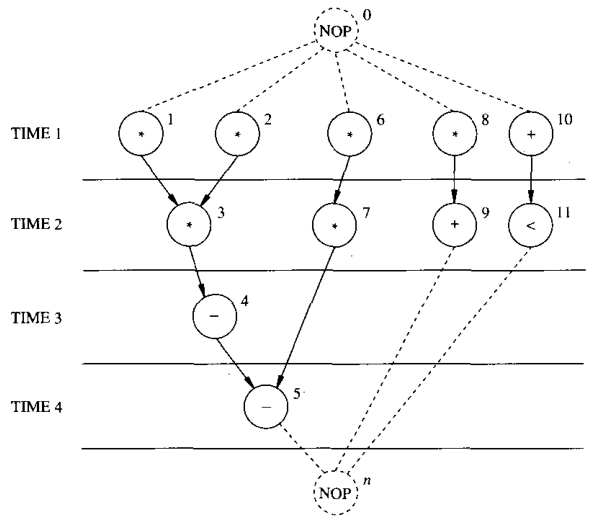
\includegraphics[width=\textwidth]{./Cap3/Images/Image17.png}
    \end{subfigure}
    \quad\quad\quad
    \begin{subfigure}[b]{0.4\textwidth}
        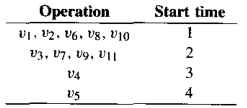
\includegraphics[width=\textwidth]{./Cap3/Images/Image18.png}
    \end{subfigure}
    \caption[Optional caption]{Scheduled  sequencing  graph. The latency of the schedule is $ \lambda=t_{n}-t_{0} = 5-1=4 $}
    \label{fig:ExaSeq}
\end{figure}
\begin{figure}[H]
    \centering
    \begin{subfigure}[b]{0.3\textwidth}
        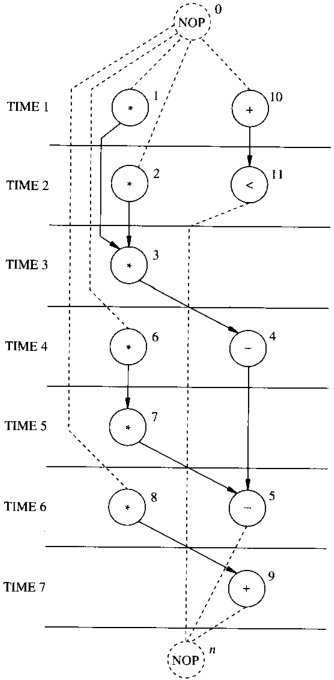
\includegraphics[width=\textwidth]{./Cap3/Images/Image19.png}
    \end{subfigure}
    \quad\quad\quad
    \begin{subfigure}[b]{0.4\textwidth}
        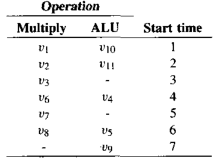
\includegraphics[width=\textwidth]{./Cap3/Images/Image20.png}
    \end{subfigure}
    \caption[Optional caption]{Scheduled  sequencing  graph  under  resource constraints. The latency of the schedule is $ \lambda=t_{n}-t_{0} = 8-1=7 $}
    \label{fig:ExaSeqCons}
\end{figure}

\subsection{The  Spatial Domain: Binding}
Let us consider now the relations among operations and resources. We define the type  of an operation as the type of computation it performs. It may be an arithmetic operation, such as addition or multiplication, or an application-specific operation, such as evaluating a Boolean function.\\
It is interesting to note that there may be more than one operation with the same type. In this case \textit{resource sharing}  may be applied. Conversely, the binding problem can be extended to a resource \textit{selection problem} by assuming that there may be more than one resource applicable to an operation.\\
A  fundamental concept that relates operations to resources is  \textit{binding}. It specifies which resource implements an operation. A  simple case of binding is  a  dedicated resource. Each operation is bound to
one resource, and the resource binding is  a  one-to-one function.\\
A  resource binding may associate one instance of a resource type to more than one operation. In this case, that particular resource is  shared  and binding is a many-to-one function.  A  necessary condition for  a  resource binding to produce a valid circuit implementation is that the operations corresponding to a shared resource do not execute concurrently. A  resource binding can  be  represented by a  labeled hypergraph.
\begin{figure}[H]
	 \centering
	 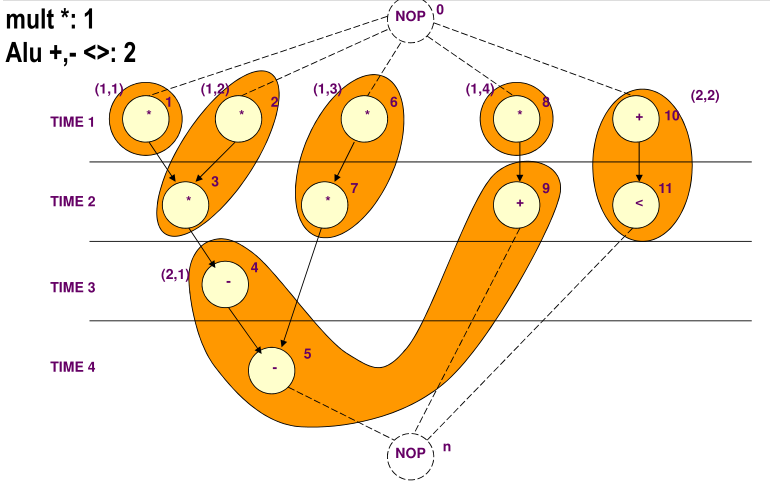
\includegraphics[width=0.5\textwidth]{./Cap3/Images/Image21.png}
	 \caption[Optional caption]{Labeled hypergraph}
	 \label{fig:hypergraph}
\end{figure}

\subsection{Resources}
Resources implement different types of functions in hardware. They can be broadly classified as follows:
\begin{itemize}
\item \textit{Functional resources}  process data. They implement arithmetic or logic functions
\item \textit{Memory resources}  store data. Examples are registers and memory.
\item \textit{Interface resources}  support data transfer. Interface resources include busses that may he used as a major means  of  communication inside a data path.
\end{itemize}